\documentclass[12pt,a4paper,titlepage]{report}
\usepackage[utf8]{inputenc}
\usepackage[german]{babel}
\usepackage[T1]{fontenc}
\usepackage{amsmath}
\usepackage{amsfonts}
\usepackage{hyperref}
\usepackage{csquotes}
\usepackage{amssymb}
\usepackage{ragged2e}
\usepackage{graphicx}
\usepackage{pgfplots}
\usepackage[applemac]{inputenc}
\usepackage[backend=biber, sorting=none]{biblatex}
\usepackage{hyperref}
\addbibresource{lit.bib}
\author{Frank Röder 6526113, Julius Plehn 6535163}
\title{Simulation der Ausbreitung von Schallwellen in einem dreidimensionalen Raum}
\begin{document}
	\begin{titlepage}
		\raggedleft\textbf{\Huge Simulation der Ausbreitung von Schallwellen in einem dreidimensionalen Raum}\\
		\vspace{\fill}
		\centering Frank Röder, Julius Plehn
	\end{titlepage}
	\tableofcontents. 
\begin{abstract} 
Zusammenfassung
 \end{abstract}
\chapter{Problemstellung}
Da es sich in der Realit{\"a}t als sehr unpraktisch erweist, wenn man Lautsprecher in einem gro{\ss}en Raum mehrmals umplatzieren muss, durch wiederholtes ausprobieren, hinh{\"o}ren und erneutes umstellen nicht gerade schnell zu einem guten Ergebnis kommt, haben wir uns als Ziel gesetzt ein Modell zur Simulation von Schall in einem 3-dimensionalen Raum zu entwicklen. 
\\
Die wichtigen Eigenschaften, wie die Interferenz, Reflexion und das Ausl{\"o}schen haben wir uns zur Aufgabe gemacht. Wir wollen Schallwellen darstelle, indem wir \dq Frequenzteilchen\dq  wellenartig sich im Raum bewegen lassen. Als m{\"o}gliches Szenario hat man nun 2 Quellen, von denen Schall ausgeht. M{\"o}gliche Hindernisse und W{\"a}nde sollen sich auf das Verhalten des Schalls auswirken. Zudem kann es noch Hindernisse geben, die die Verteilung im Raum beeintr{\"a}chtigt und zu unterschiedlichsten Erkenntnissen f{\"u}hren. Durch die angestrebte Visualisierung k{\"o}nnte man nun die kritischen Stellen, bei denen sich besonders viel Schall ausl{\"o}scht erkennen, das gegebene Szenario modifizieren und das Ereignis erneut durchlaufen. Nach langer {\"U}berlegung und Recherche haben wir uns schlussendlich auf eine sehr einfache abstrakte Weise geeinigt, die uns nicht zu sehr von unseren eigentlichen Parallelisierungszielen abbringt und eine Idee von der Realit{\"a}t gibt. Jedoch wird nicht das vollkommene physikalische Wesen des Schalls widerspiegelt. Da man sich dabei auf hohe Mathematik besinnen kann, beschr{\"a}nken wir uns auf die genannte Modellierung und gehen auf eine m�glichst genaue Aufl{\"o}sung ein, bei der auch ein hoher Rechneraufwand entsteht.
Ein weiteres Problem war die Umsetzung der Idee. Die Frage nach Datenstrukturen zur Speicherung und zur Speicherung der \dq Frequenzteilchen\dq. Des Weiteren stehen einem auch noch sehr viele physikalische Formeln zu verf{\"u}gung, die das Verhalten viel genauer beschreiben, jedoch mehr physikalischen Verst{\"a}ndnis bed{\"u}rfen und dann auch noch korrekt in ein Programm integriert werden m{\"u}ssten. Von Gesetzten und der Eigenschaft des Mediums Luft, kreisten die Gedanken um den Zeitplan , um die neue Programmiersprache und die m{\"o}glichen Arbeitsaufteilungen f{\"u}r die Prozesse.
Folgende Grafik soll die Idee der Teilchen beschreiben, die pro Zeiteinheit eine bestimmte Lautst{\"a}rke(dB) des jeweiligen Frequenzbereiches haben.
\n
\begin{figure[h]}
\centrering
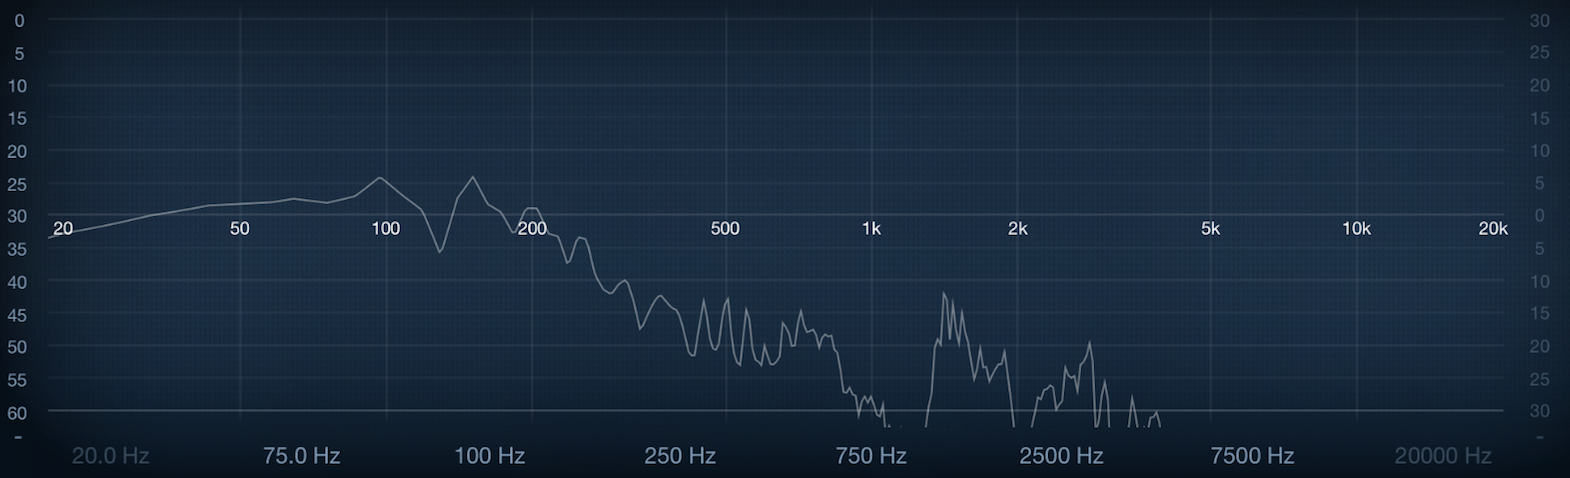
\includegraphics[width= 14cm]{eq}
\caption{\\Frequenzgang in einem Equalizer}
\end{figure}
\chapter{Lösungsansatz}
Um der Problemstellung her zu werden, haben wir uns {\"u}berlegt eine einfache 3-D Matrix in C zu nehmen, in der wir pro Eintrag einen Pointer (auf ein Item), welcher auf ein struct zeigt, ablegen. Das struct wiederum besteht in Falle eines \dq Sounds \dq mit der id = 0 aus 10 Frequenzbereichen mit einer vorgegeben Ausbreitungsrichtung. Zudem machen wir auch mit der id =  1 kenntlich, wenn es sich um ein Hindernis handelt. Da wir hierbei auf das Problem stie{\ss}en, bei mehrfachen Eintr{\"a}gen weitere Matrizen zur Speicherung der {\"U}berlagerung zu reservieren, haben wir uns auf "Doppelt-Verkettete-Listen" geeinigt, die nun in jedem Matrixeintrag i,j,k bestehen. In einer solchen verketteten Liste kommen nicht �berdurchschnittlich viele Eintr{\"A}ge vor, da wir nach jeder Verschiebung sofort die {\"U}berlagerung verrechnen und die Liste wieder entlasten.
Schlussendlich arbeiten wir mit 2 identischen Matrizen. In der ersten stehen die vorhanden Elementen, in der 2. schreiben wir nun die Teilchen nach ihrer Bewegung hinein, somit dient sie als Puffer f{\"u}r die Verschiebung. Man kann Sounditems und Hindernisse an beliebiger Position erstellen und eine Richtung zuweisen in die sich der Sound bewegen soll.
Bei der Bewegung erstellen wir durch eine Funktion Nachbarelemente, welche eine \dq Welle \dq formen sollen. Zur Feststellung ob ein Teilchen verschoben werden soll, gehen wir in einer 3-fach verschachtelten For-Schleife den Raum je Programmablauf i-mal durch und {\"u}berpr{\"u}fen jeden Eintrag auf n{\"o}tige Operationen. Dieses wiederholen wir hunderte Male, je nachdem wie viele Schritte die  Visualisierung von uns verlangt, um ein sch{\"o}nes Ergebnis zu erhalten. 

\chapter{Parallelisierungsschema}
Um Objekte in einem dreidimensionalen Raum zu paralllelisiern, bietet es sich an, den Raum in kleinere, möglichst unabhängige, Bereiche einzuteilen. Die Unabhängigkeit der einzelnen Bereiche reduziert die Kommunikation der Prozesse und vereinfacht die Programmierung enorm. Im folgenden ein kleines Beispiel:  Angenommen wir unterteilen den Raum an der X-Achse entlang, dann haben wir einzelne Abschnitte, die alle die gleichen Y \& Z Ausmaße besitzen. Lediglich die X Ausmaße unterscheiden sich (maximal um 1). Diese Verteilung übernimmt der Prozess 1 (MPI Task 0). Nach dieser Aufteilung wird den Simulationsprozessen eine Konfiguration geschickt. Diese beinhaltet für alle die gleichen Y und Z Grenzen, die eben berechneten X Grenze und einen Offset für die Visualisierung. Des weiteren verteilt der Master nicht nur die Aufgaben, sondern er fungiert auch als Taktgeber. Diesen brauchen wir desshalb, da die Prozesse, die ihre aufgeteilten Räume berechnen, in unterschiedlich Stadien wären. Das würde die ganze Simulation sinnlos machen, da das Resultat nicht einer unparallelisierten Berechnung entsprechen würde, sondern vollkommen verzerrt wäre. Neben diesem Masterprozess gibt es noch einen extra Prozess für die Visualisierung. Dieser wird ebenfalls von dem Masterprozess synchronisiert, sodass er in jedem Durchlauf die zu visualisierenden Daten von den anderen Prozessen erwartet. Die Simulationsprozesse senden nach jedem Durchlauf ihre Feldbelegungen an die Visualisierung. Dazu addiert jede Simulation ihre X Grenze mit dem in der Startkonfigurierung mitgeteilten X Offset. Hieraus ergibt sich wieder die Koordinate in dem Gesamtraum, sodass wieder ein großes Gebild entsteht. Der Visualisierungsprozess speichert diese Informationen in einer JSON Datei, die mit dem Javascript Visualizer abgebildet werden kann.\\
\\Da die einzelnen Tonelemente wandern, kann es auch vorkommen, dass Elemente ihren Prozess verlassen müssen. Wie mit diesen Elementen verfahren werden muss unterscheidet sich durch ihre Richtung. Wenn Elemente also über ihre Y oder Z Grenzen treten (und hierbei nicht auf eine Wand stoßen), wird das jeweilige Element entfernt. Sollte ein Element jedoch ihre X Grenze übertreten, so bedeutet das, dass das Element an einen Nachbarprozess übergeben werden muss. Hierbei muss beachtet werden, dass der Erste Simulationsprozess nur an der rechten Seite einen Nachbarn hat und das der letzte Prozess nur Links einen Nachbarn hat. Alle anderen Prozesse besitzen zwei Nachbarn. Diese Spezialfälle werden also gesondert bearbeitet. Ab der zweiten Iteration, die durch den Masterprozess veranlasst wird, wird von den Nachbarn ein Array mit neuen Tonelementen erwartet. Mit diesen erhaltenen Informationen wird dann ein neues Element mit den alten Spezifikationen generiert. Dem entsprechend wird am Ende jeder Iteration, also nachdem alle Elemente verschoben und behandelt wurden, ein Array mit allen zu sendenen Elementen an die Nachbarn weitergegeben. Diese empfangen das Array am Anfang der nächsten Iteration. Da es linke und rechte Nachbarn gibt werden auch zwei unterschiedliche Arrays f�r die Kommunikation erzeugt.
\chapter{Laufzeitmessung}
Durch Messungen des sequenziellen Programms konnten wir ein sinnvolles Ma{\ss} der Arbeit , die ein Prozess verrichten soll, ermitteln. Diese Erkenntnisse sollen uns sp{\"a}ter bei der Parallelsierung das Verh{\"a}ltnis von Prozessen und Raumgr{\"o}{\ss}e helfen.
\\
\begin{figure[b]}
\centrering
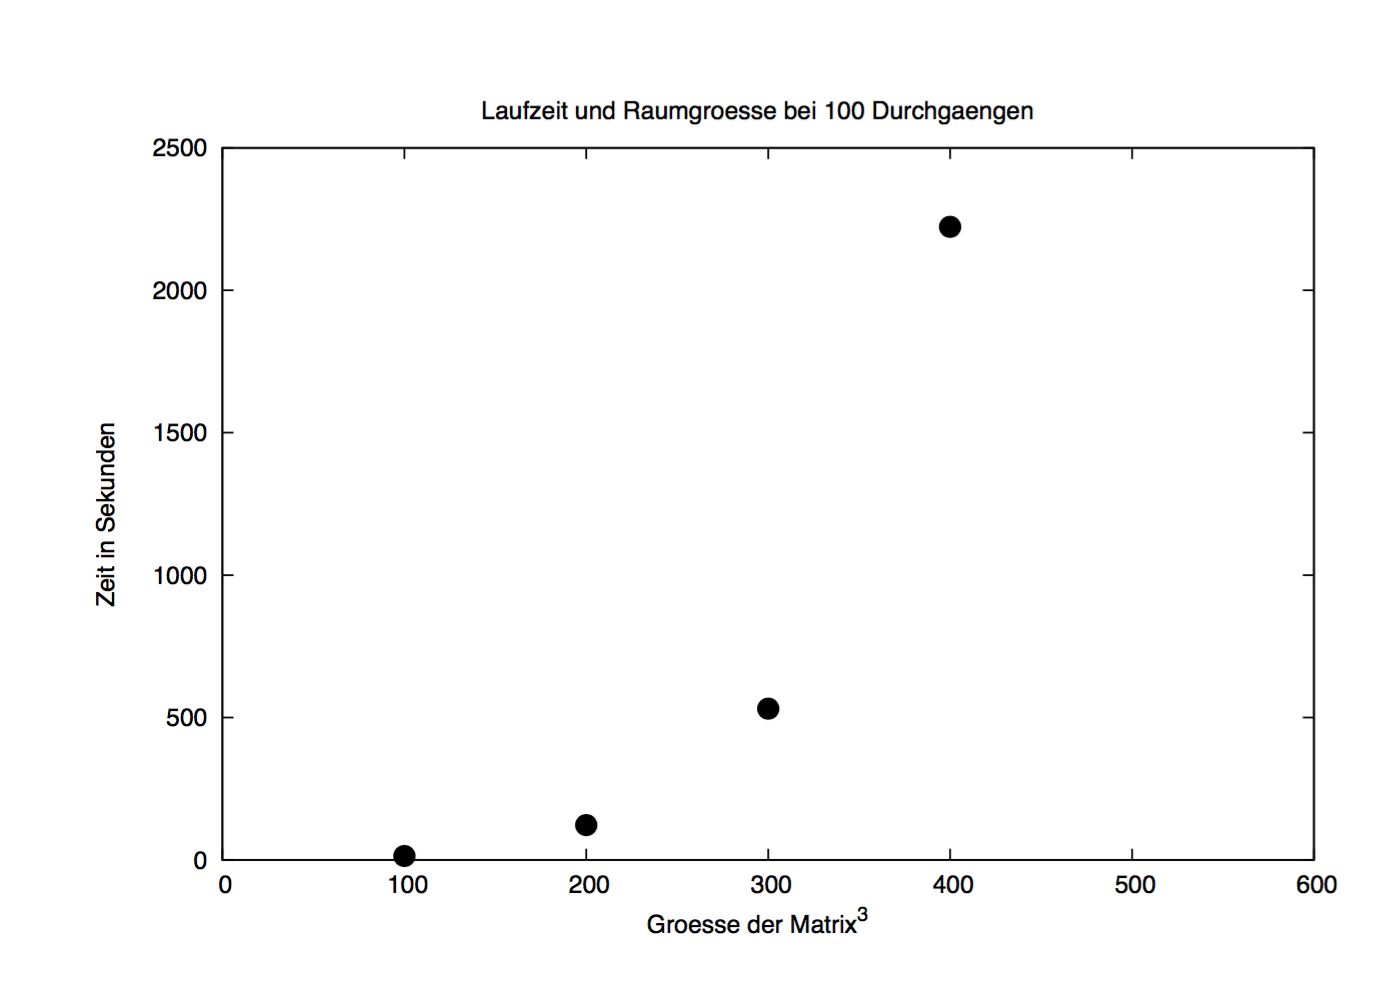
\includegraphics[width= 12cm]{laufzeit1}
\end{figure}
\newpage
Die folgende Grafik zeigt die Laufzeit bei gegebener Anzahl an Prozessen um den Raum zu durchlaufen und jede Zelle auf ihren Zustand zu {\"u}berp{\"u}fen.
\begin{figure[c]}
\centrering
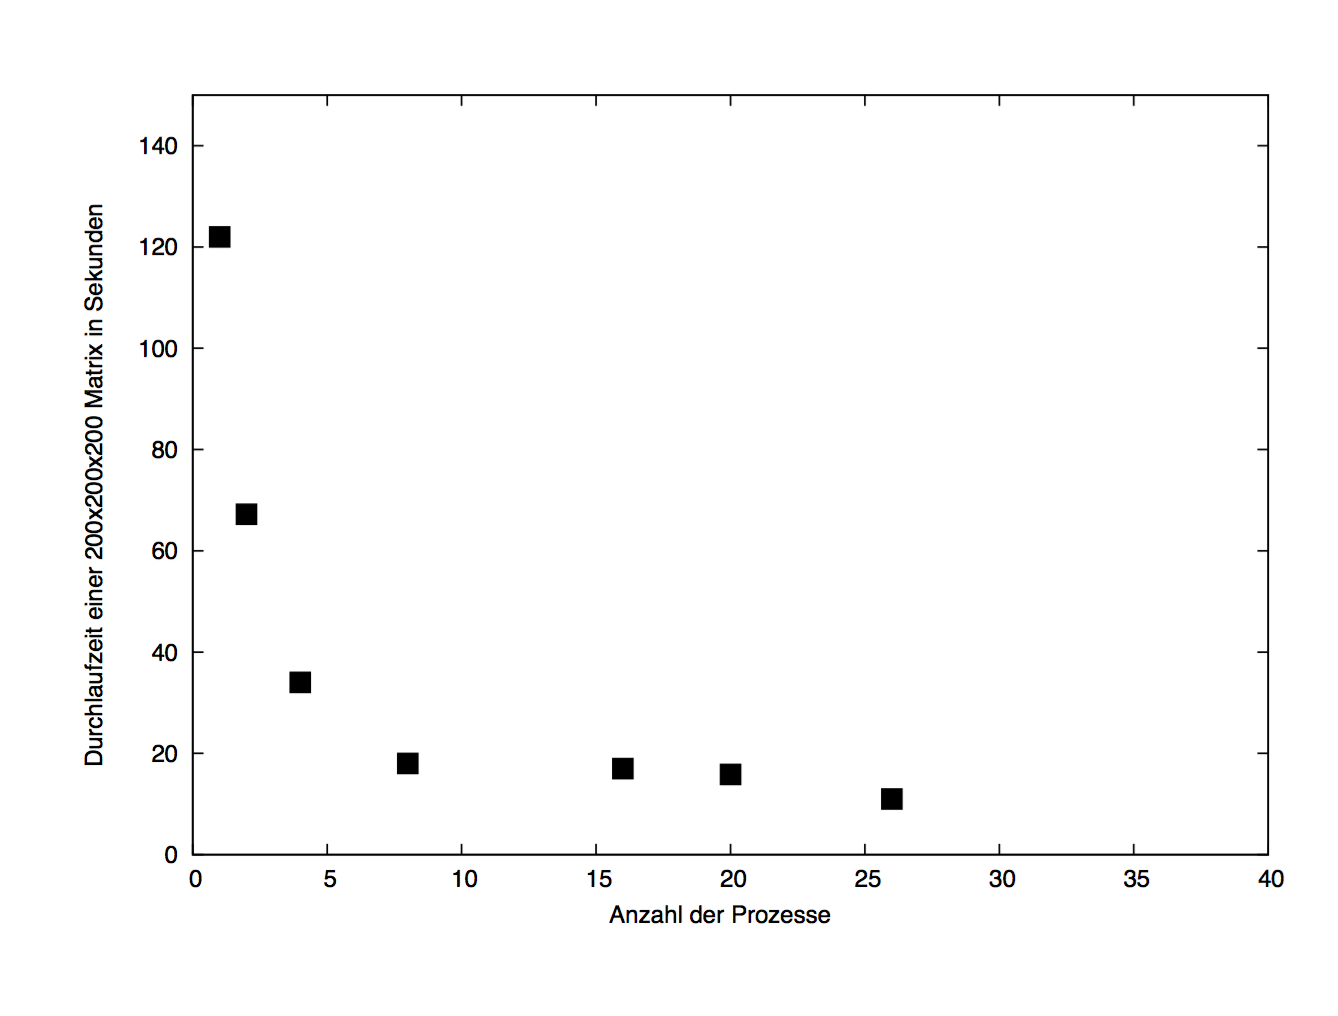
\includegraphics[width= 12cm]{paraextime}
\end{figure}
\chapter{Leistungsanalyse} Hierbei handelt es vom Trade-Off zwischen Anzahl an Prozessen, die in Richtung der X-Achse kommunizieren m{\"u}ssen.
\chapter{Skalierbarkeit}
Nach unserer Idee kann man einen belieb gro{\ss}en Raum f{\"u}r die  Simulation nutzen, da jeder Prozess f{\"u}r sich einen kleinen Raum bearbeitet und durch die Aufteilung der X-Achse maximal 2 Nachbarn hat.
\chapter{Programmausgabe}
\chapter{Fazit und Zukunft}
Das Praktikum erwies sich als eines der lehrreichsten Module, die wir je belegt haben. Wir haben sehr viel Spa{\ss} gehabt und gleichzeitig viel gelernt, denn aus eigenen Fehlern und aus der Erfahrung die man durch Erkunden der neuen Umgebung macht, erntet man gro{\ss}e Fr{\"u}chte an Wissen. Auch die M{\"o}glichkeit an der Universit{\"a}t sich an einem Projekt auszuprobieren ist wohl der letzte Zeitpunkt in dem Fehler noch tolerierbar sind. Oft haben wir uns mit nicht zu erwartenden Fehlern der Speicherreservierung in C herumgeschlagen. Dieses nahm nicht nur sehr viel Zeit in Anspruch, sondern forderte auch das Denken {\"u}ber das Zeitmanagement. Haben wir uns zu lange mit einer Sache aufgehalten, gab es gl{\"u}cklicherweise noch einen Plan B, der uns f{\"u}rs erste wieder vern{\"u}nftig an dem Projekt weiter arbeiten lies. Das was fehlte war noch ein Plan C, denn wenn einem die Probleml{\"o}sungen ausgehen, dann wird auch der Zeitdruck h{\"o}her m{\"o}glichst schnell die L{\"o}sung zu finden. Umso mehr haben wir uns gefreut, wenn ein solches Hindernis nicht wiederkehrend beseitigt wurde.
Insgesamt haben wir sehr viel Zeit ben{\"o}tigt um uns immer wieder in Vorgehen einzulesen und Erfahrung darin zu sammeln, wie man die Meldungen der Debugger interpretiert. \\
{\raggedright
 \printbibliography
}
\end{document}
